\documentclass{beamer}
\usetheme{Boadilla}
\usepackage{essay-def}
\usepackage{bm}
\usepackage{amsfonts}
\usepackage{amssymb}
\usepackage{amsmath}
\usepackage{amsthm}
\usepackage{comment}
\usepackage{geometry}
\geometry{left=1cm,right=1cm}
\title[Interview for NUS]{Interview for NUS}
\author{Jiaxi Zhao (Stony Brook University)}
\institute[]{}
\date{July 2021}
\begin{document}
\par \setlength{\parindent}{2em}

\begin{frame}
\titlepage
\end{frame}


\begin{frame}{Distances on probability space}
    \begin{figure}[H]
          \centering
          \centerline{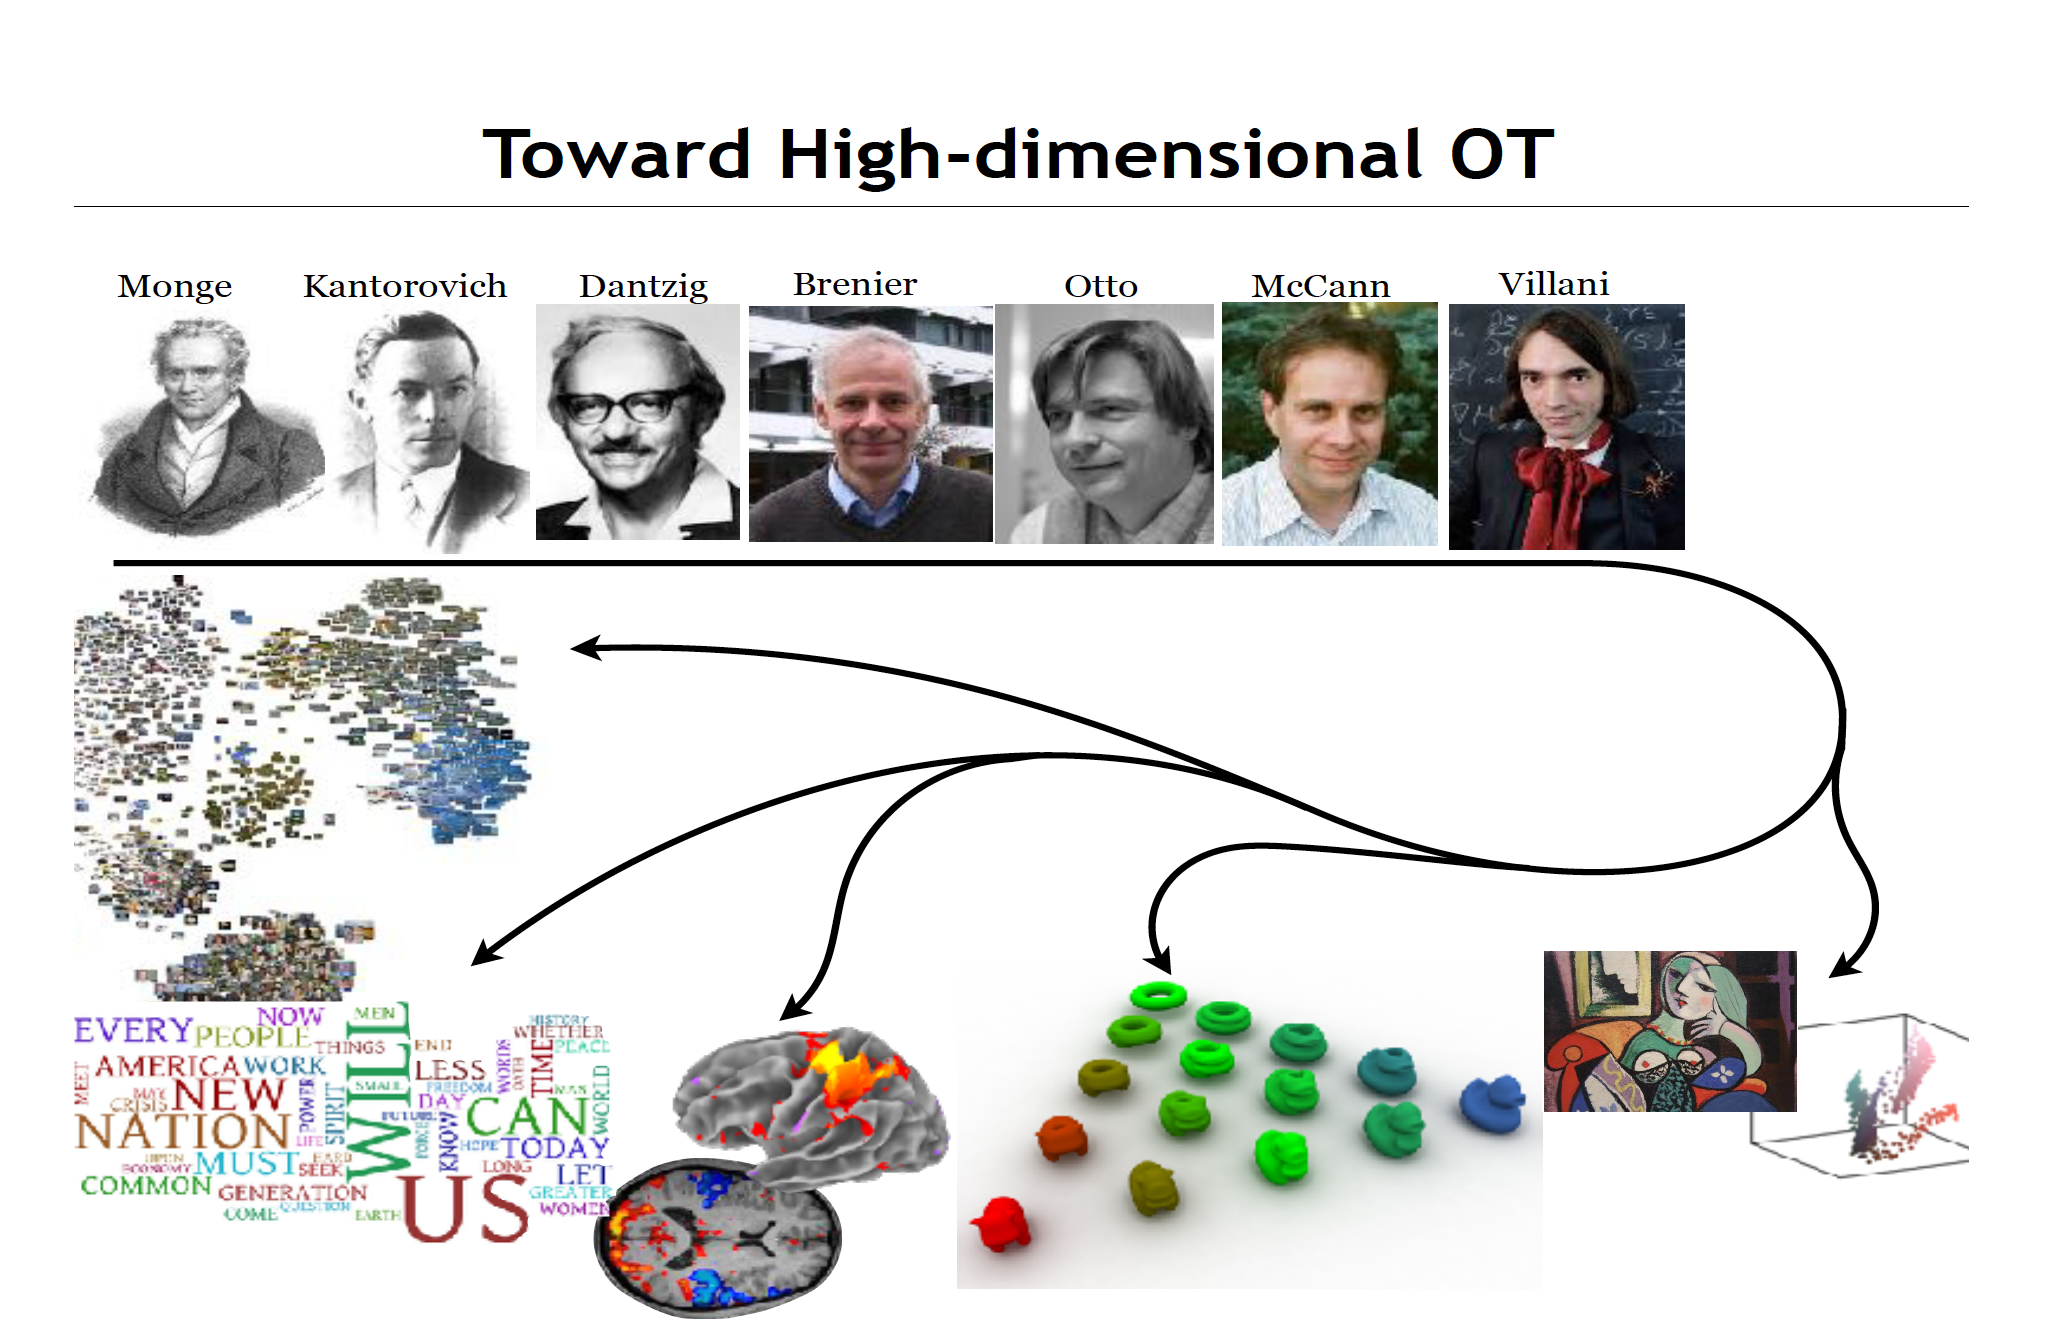
\includegraphics[width=0.6\linewidth]{history.png}}
  %        \caption{History of statistics and geometry}
        \end{figure}
\end{frame}


\begin{frame}{Statistical information matrix}

    \begin{definition}[Statistical Information Matrix]
	Consider the density manifold $(\mathcal{P}(\mcX), g)$ with a metric tensor $g$, and a smoothly parametrized statistical model $ p_\theta$ with parameter $\theta\in\Theta \subset \mathbb{R}^d$. 
	Then the pull-back $G$ of $g$ onto the parameter space $\Theta$ is given by
	\begin{equation*}
	G(\theta)=\Big\langle \nabla_\theta p_\theta, g( p_\theta) \nabla_\theta p_\theta\Big\rangle.
	\end{equation*}
Denote $G(\theta)=(G(\theta)_{ij})_{1\leq i,j\leq d}$, then 
\begin{equation*}
G(\theta)_{ij}=\int_{\mathcal{X}}{\frac{\partial}{\partial \theta_i}p(x;\theta)\Big(g(p_\theta)\frac{\partial}{\partial \theta_j}p\Big)(x;\theta)}dx.
\end{equation*}
Here we name $g$ the statistical metric, and call $G$ the statistical information matrix.
\end{definition}
\end{frame}


\begin{frame}{Statistical Information Matrix}
    \begin{table}[h]
\setlength{\belowcaptionskip}{-0.cm}
\setlength{\floatsep}{0cm}
%\hspace{-4.0cm}
\centering
    \resizebox{\textwidth}{0.25\textwidth}{
\begin{tabular}{|l|c|c|}
\hline 
Probability Family & Wasserstein information matrix & Fisher information matrix \\
\hline
$
\begin{aligned}
    & \text{Uniform:}        \\
    & p(x;a,b) = \frac{1}{b - a}\mathbf{1}_{(a,b)}(x)
\end{aligned} $
 & $G_W(a,b) = \frac{1}{3} \begin{pmatrix}
1 & \frac{1}{2}\\
\frac{1}{2} &  1
\end{pmatrix}$ & $G_F(a,b)$ not well-defined 
\\
\hline
$
\begin{aligned}
    & \text{Gaussian:}        \\
    & p(x;\mu,\sigma)=\frac{e^{-\frac{1}{2\sigma^2}(x-\mu)^2}}{\sqrt{2\pi} \sigma}
\end{aligned}$ & $G_W(\mu,\sigma)=\begin{pmatrix}
1& 0 \\
0 &  1
\end{pmatrix}$ &  $G_F(\mu,\sigma) = \begin{pmatrix}
			\frac{1}{\sigma^2} & 0		\\
			0 & \frac{2}{\sigma^2}
		\end{pmatrix}$    
\\
\hline
$
\begin{aligned}
    & \text{Exponential:}        \\
    & p(x;m,\lambda) = \lambda e^{-\lambda\lp x - m \rp}
\end{aligned}$
& $G_W(m,\lambda)=\begin{pmatrix}
    1 & \frac{1}{\lambda^2}     \\
    \frac{1}{\lambda^2} & \frac{2}{\lambda^4}
\end{pmatrix}$ & $G_F(m,\lambda)$ not well-defined 
\\    
\hline
$
\begin{aligned}
    & \text{Laplacian:}        \\
    & p(x;m,\lambda) = \frac{\lambda}{2}e^{-\lambda|x-m|}
\end{aligned}
 $ & $G_W(m,\lambda)=\begin{pmatrix}
    1 & 0     \\
    0 & \frac{2}{\lambda^4}
\end{pmatrix}$ & 
$G_F(m,\lambda) = \begin{pmatrix}
			\lambda^2 & 0		\\
			0 & \frac{1}{\lambda^2}
		\end{pmatrix}$ 
\\    
\hline
$\begin{aligned}
    & \text{Location-scale:}        \\
    & p(x;m,\lambda) = \frac{1}{\lambda}p(\frac{x - p}{\lambda})
\end{aligned}$ & $G_W(\lambda,m)=\begin{pmatrix}
    \frac{\mathbb{E}_{\lambda,m}x^2-2m\mathbb{E}_{\lambda,m}x+m^2}{\lambda^2} & 0     \\
    0 & 1
\end{pmatrix}$ & 
$G_F(\lambda,m) = \begin{pmatrix}
			\frac{1}{\lambda^2} \lp 1 + \int_{\mbR} \lp \frac{\lp x - m \rp^2 p'^2}{\lambda^2 p} + \frac{\lp x - m \rp p'}{\lambda}\rp dx  \rp & \int_{\mathbb{R}}  \frac{(x - m)p'^2}{\lambda^3p} dx		\\
			\int_{\mathbb{R}}  \frac{(x - m)p'^2}{\lambda^3p} dx & \frac{1}{\lambda^2}\int_{\mathbb{R}} \frac{p'^2}{p} dx
		\end{pmatrix}$ 
		\\    
\hline
$
\begin{aligned}
    & \text{Independent:}        \\
    & p(x,y;\theta) = p(x;\theta)p(y;\theta)
\end{aligned}
 $ & $G_W(x,y;\theta)=G_W^1(x;\theta)+G_W^2(y;\theta)$ &
$G_F(x,y;\theta)=G_F^1(x;\theta)+G_F^2(y;\theta)$    \\    
\hline
$
\begin{aligned}
    \text{ReLU} &\text{ push-forward:}        \\
    & p(x;\theta) = f_{\theta*}p(x), \\ f_{\theta} \ \theta&\text{-parameterized ReLUs.}.
\end{aligned}
 $ & $G_W \lp \theta \rp= F\lp \theta \rp$, $F$ cdf of $p(x)$ &
$G_F(\theta)$ not well-defined   \\    
\hline
\end{tabular}}
\label{table1}
\caption{In this table, we present Wasserstein, Fisher information matrices for various probability families.}
\end{table}
\end{frame}


\begin{frame}{Wasserstein-Cramer-Rao bound}
\begin{theorem}[Wasserstein-Cramer-Rao inequalities]\label{WCR}
Given any set of statistics $T = \left( T_1,...,T_n\right) \colon \mathcal{X}\rightarrow \mathbb{R}^n$, where $n$ is the number of the statistics, define two matrices $\mathrm{Cov}^W_\theta[T(x)]$, $ \nabla_\theta \mathbb{E}_{p_\theta} [T(x)]^{T}$ as below:
\begin{equation*}
    \mathrm{Cov}^W_\theta[T(x)]_{ij} = \mathrm{Cov}^W_\theta[T_i,T_j], \qquad \nabla_\theta \mathbb{E}_{p_\theta} [T(x)]^{T}_{ij} = \frac{\pa}{\pa \theta_j} \mathbb{E}_{p_\theta} [T_i(x)],
\end{equation*}
then
\begin{equation*}
\mathrm{Cov}^W_\theta[T(x)] \succeq \nabla_\theta \mathbb{E}_{p_\theta} [T(x)]^{T}G_W(\theta)^{-1}\nabla_\theta \mathbb{E}_{p_\theta} [T(x)]. 
\end{equation*}
\end{theorem}
\end{frame}


\begin{frame}{Poincare online efficiency }
\scriptsize
\begin{corollary}[Poincare Efficiency]\label{WFNE}
For the dynamics
\begin{equation*}
    \theta_{t+1} = \theta_t - \frac{1}{t}\nabla_{\theta}^W l(x_t,\theta_t),
\end{equation*}
where $l(x_t,\theta_t) = \log p\lp x_t, \theta_t \rpz$ is the log-likelihood function. The Wasserstein covariance updates according to
\begin{equation*}
	\begin{aligned}
	V_{t+1} = & \ V_t + \frac{1}{t^2} G_W^{-1}(\theta_*) \mbE_{p_{\theta_*}} \lb \nabla_x \lp \nabla_{\theta}l(x_t,\theta_*) \rpz \cdot \nabla_x \lp \nabla_{\theta}l(x_t,\theta_*)^{T} \rpz  \rb G_W^{-1}(\theta_*)  \\
& \ - \frac{2}{t} V_t G_F (\theta_*) G_W^{-1} (\theta_*) + O\left( \frac{1}{t^3} \right) + o\lp \frac{V_t}{t} \rpz .
	\end{aligned}
\end{equation*}
Now suppose that $\alpha = sup \{ a | G_F \succeq a G_W \}$. Then the dynamics is characterized by
\begin{equation*}\label{Poincare}
    \begin{aligned}
        V_t & = \lbb 
        \begin{aligned}
            & \ O\lp t^{-2\alpha} \rpz,  \qquad \qquad \qquad \qquad \qquad \qquad \qquad \qquad \qquad \  2\alpha \leq 1,   \\
            & \  \frac{1}{t}\lp 2G_FG_W^{-1} - \mfI \rpz^{-1}{G_W^{-1}(\theta_*) \mcI  G_W^{-1}(\theta_*) } + O\lp \frac{1}{t^2} \rpz, \quad 2\alpha > 1,
        \end{aligned}\right.
        \end{aligned}
        \end{equation*}
where \begin{equation*}
        \mcI = \mbE_{p_{\theta_*}} \lb \nabla_x \lp \nabla_{\theta}l(x_t,\theta_*) \rpz \cdot \nabla_x \lp \nabla_{\theta}l(x_t,\theta_*)^{T} \rpz  \rb.
\end{equation*}
\end{corollary}
\end{frame}


\begin{frame}{Scaling limit of the Gaussian mixture model (GMM)}
	Gaussian mixture models (GMM) are widely used in statistical inference 
	%\footnote{Huber, On Entropy Approximation for Gaussian Mixture Random Vectors, 2008} 
	(statistical models) and scientific computation.
	%\footnote{Jianfeng Lu, Numerical methods for stochastic differential equations based on Gaussian mixture, 2018}.
	\par
	A simple review of GMM:
	\bequn
	\begin{aligned}
	\rho: \Theta & \rightarrow \mcP\lp \mbR \rp, \quad \Theta \subset \mbR^{N - 1},			\\
	\theta & \mapsto \rho_{\theta} = \sum_{i = 1}^{N - 1} \theta_i \lp \rho_{i + 1} - \rho_i \rp + \rho_1 = \sum_{i = 1}^{N} p_i\rho_i, \\
	1  & = \theta_0 > \theta_1 > \cdots > \theta_{N - 1} > \theta_N = 0,			\\
	\rho_i & \sim \mcN\lp \mu_i, \sigma^2 \rp, \ \mu_1 < \mu_2 < \cdots < \mu_{N - 1} < \mu_N,
	\end{aligned}
	\eequn
	This work is based on the consideration of GMM.
\end{frame}


\begin{frame}{Our approach}
	We focus on the one-dimensional sample space to utilize the explicit formula for Wasserstein metric.
	\par
	\textbf{Step 1}: Define a (Fisher-Rao/Wasserstein) pull-back metric $G_W\lp \theta; \sigma \rp$ on GMMs, where $\theta$ is parameter and $\sigma$ is the variance.
	\begin{figure}[H]
          \centering
          \centerline{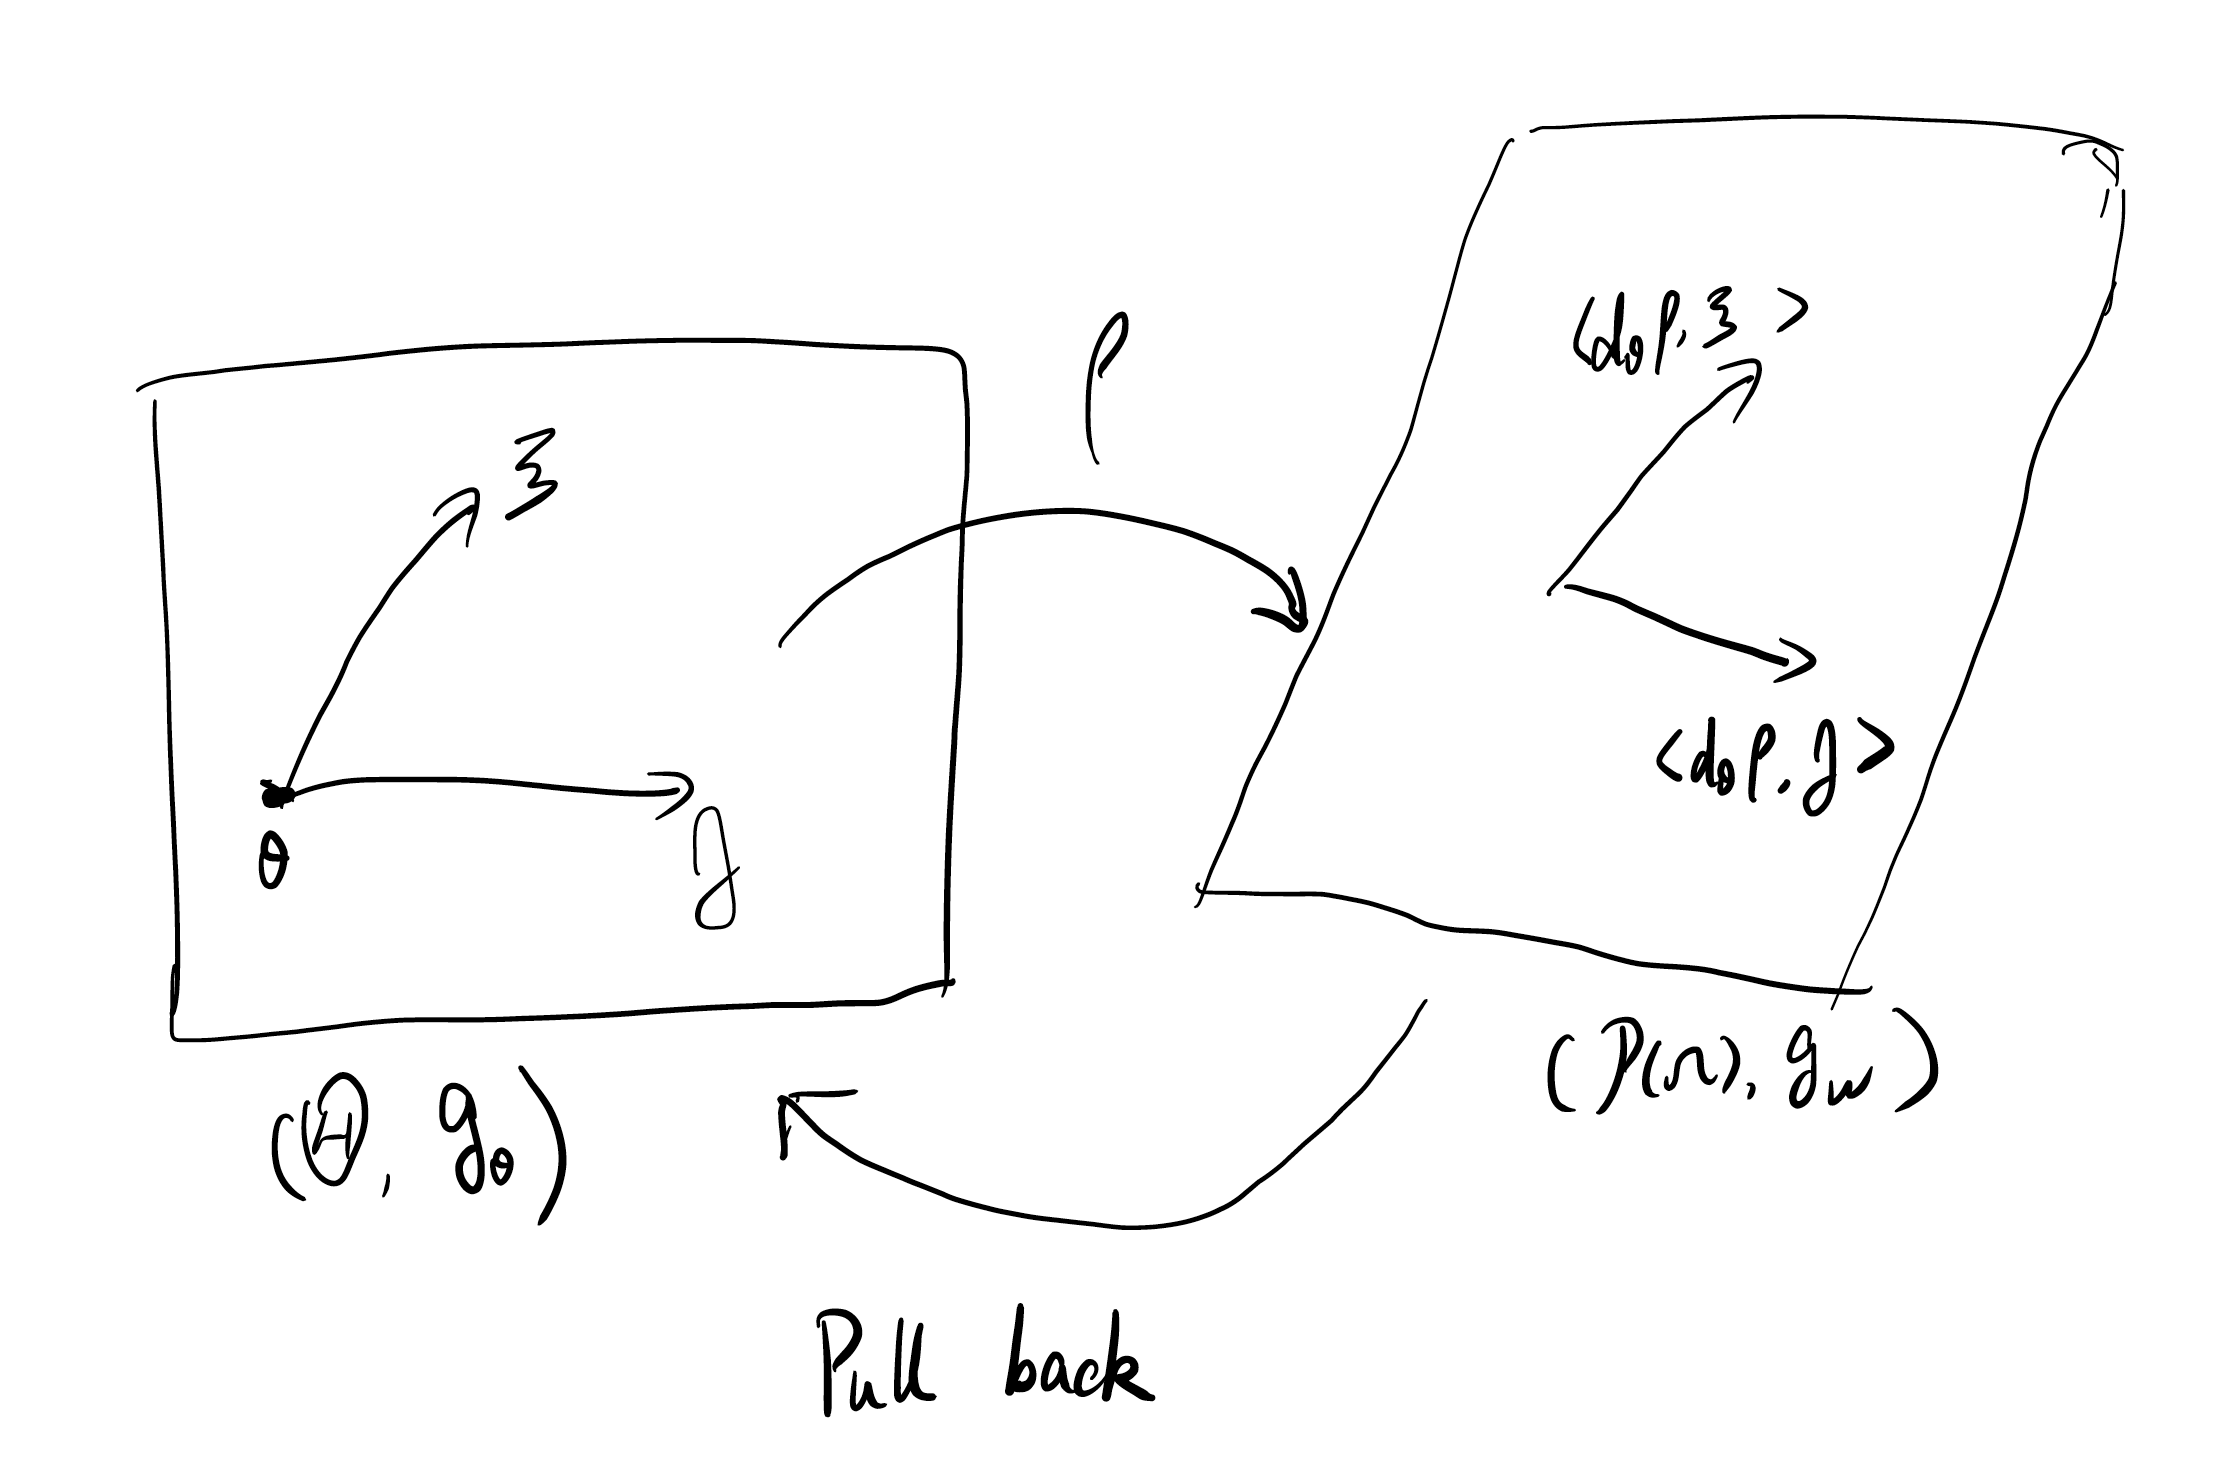
\includegraphics[width=0.7\linewidth]{pull_back.png}}
          \caption{Pull-back of the metric}
    	\end{figure}
\end{frame}


\begin{frame}{Our approach}
	\textbf{Step 2}: Rescale GMMs to approximate discrete spaces. As the variance of Gaussian tends to $0$, distributions weakly converge to a Dirac measure centered at its mean.
	\bequn
		\lim_{\sigma \rightarrow 0} \frac{G_W\lp \theta; \sigma \rp}{K\lp \sigma \rp} = G_{\wtd W}\lp \theta \rp.
	\eequn	
	\begin{figure}[H]
          \centering
          \centerline{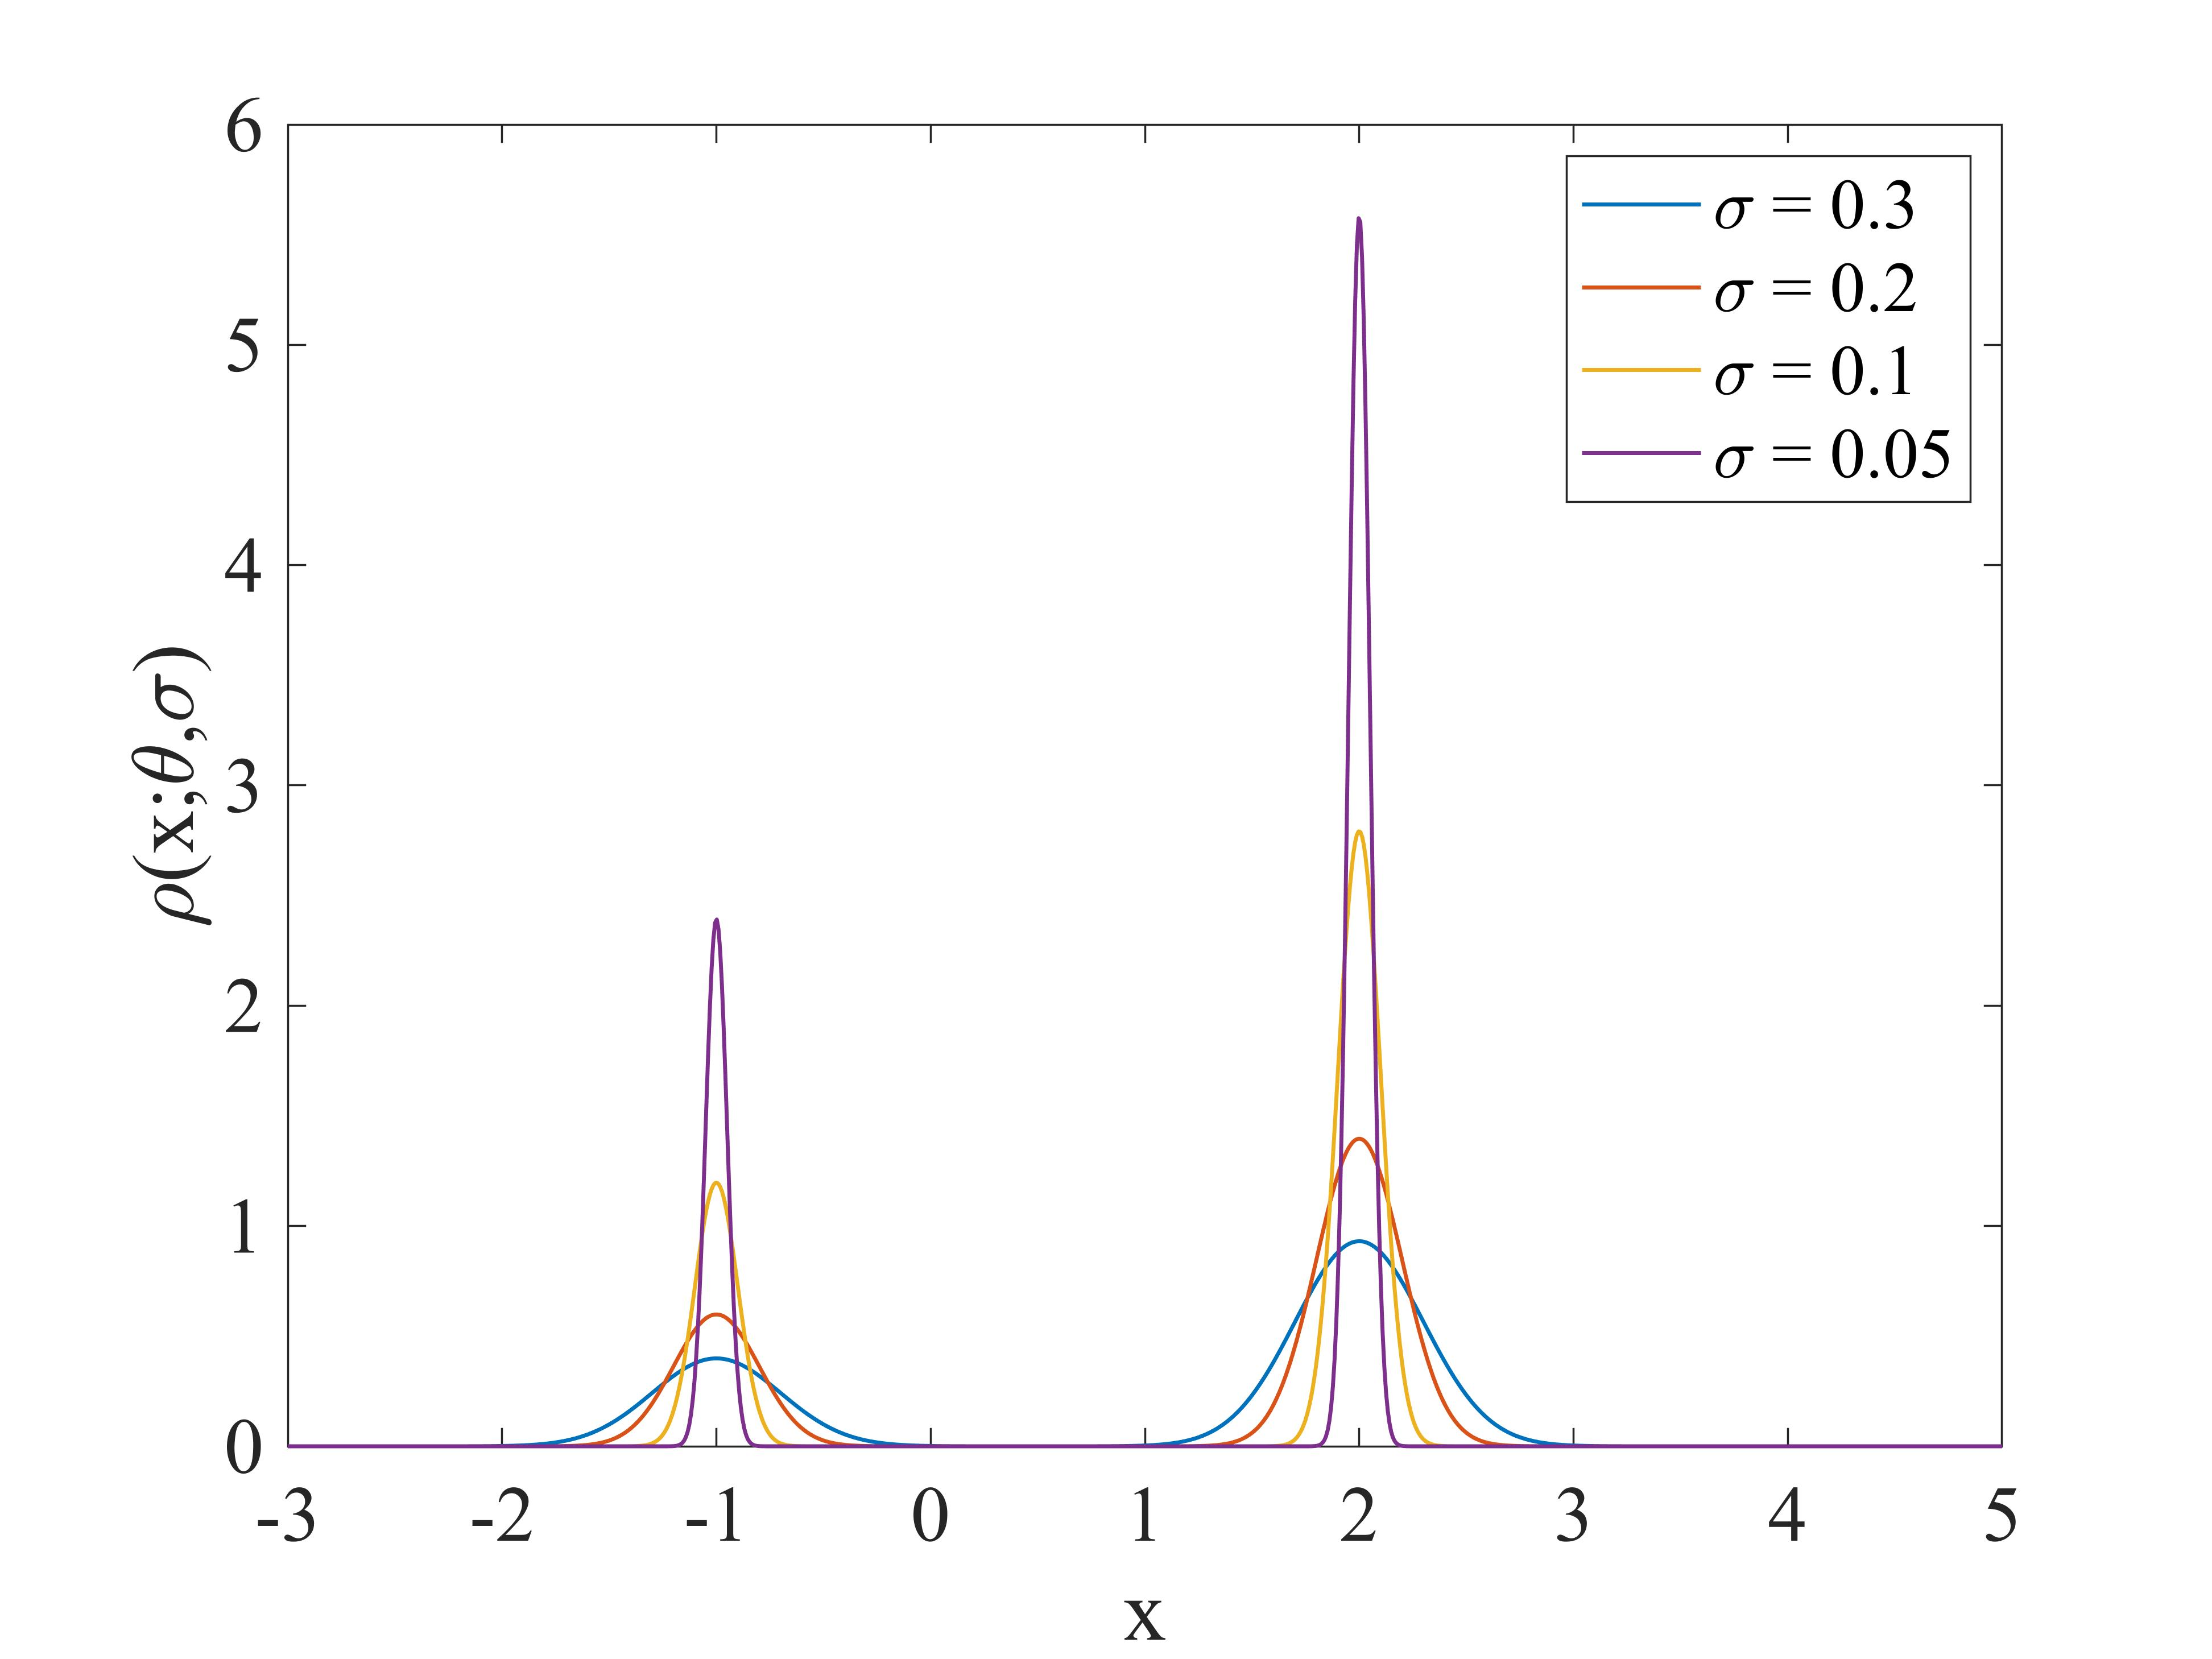
\includegraphics[width=0.55\linewidth]{Approx.jpg}}
          \caption{\scriptsize{The figure plots the density function of a family of Gaussian mixture given by $\rho\lp x \rp \sim 0.3 * \mcN\lp -1, \sigma \rp + 0.7 * \mcN\lp 2, \sigma \rp$.}}
    	\end{figure}
\end{frame}


\begin{frame}{Scaling approximation Wasserstein metric}
	\begin{Thm}[Scaling Wasserstein metric]
	For a 1-d homogeneous GMM with difference between adjacent components given by $d$, a scaling limit of Wasserstein information matrices is given by
	\scriptsize
	\bequn
		G_{\wtd W}\lp \theta \rp = \lim_{\sigma \rightarrow 0} \frac{G_W\lp \theta; \sigma \rp}{K\lp \sigma \rp} = \begin{pmatrix}
			\frac{1}{\sqrt{p_1p_{2}}} & 0 & 0 & \cdots & 0 & 0 			\\
			0 & \frac{1}{\sqrt{p_2p_{3}}} & 0 & \cdots & 0 & 0	\\
			0 & 0 & \frac{1}{\sqrt{p_3p_{4}}} & \cdots & 0 & 0			\\
			\vdots & \vdots & \vdots & \ddots & \vdots & \vdots 						\\
			0 & 0 & 0 & \cdots & 0 & \frac{1}{\sqrt{p_{N - 1}p_{N}}}
		\end{pmatrix}
	\eequn
	\normalsize
	The scaling factor appearing above is given by
	\bequn
		K\lp \sigma \rp = \sqrt{2\pi^3}\frac{\sigma^3}{d}e^{\half \lp \frac{d}{2\sigma}\rp^2}.
	\eequn
\end{Thm}
\end{frame}


\begin{frame}{Gradient flows in scaling Wasserstein geometry}	
	Following the discussion in Villani,
	%\footnote{Villani, Topics in optimal transport, 2003}, 
	we derive the gradient flow equations of potential, internal, and interaction energy functional on density manifold and scaling Wasserstein geometry
	\bequn
	\begin{aligned}
		\textbf{internal energy:} & \qquad \mcU\lp \rho \rp = \int U\lp \rho\lp x \rp \rp dx = \sum_{i = 1}^N U\lp p_i \rp,		\\
		\textbf{potential energy:} & \qquad \ \mcV\lp \rho \rp = \int V\lp x \rp d\rho = \sum_{i = 1}^N V_i p_i, 	\\
		\textbf{interaction energy:} & \qquad \mcW\lp \rho \rp = \half \int\int W\lp x - y \rp \rho\lp x \rp\rho \lp y \rp dxdy \\
		& \qquad \qquad \ \  = \sum_{i, j = 1}^N W_{ij} p_i p_j.		\\
	\end{aligned}
	\eequn	
\end{frame}


\begin{frame}{Gradient flows in scaling Wasserstein geometry}
	\small
	\bequn
	\begin{aligned}
		\textbf{internal energy:} & \quad \dot{p_i} = - \sqrt{p_i p_{i - 1} } \lp U'\lp p_i \rp - U'\lp p_{i - 1} \rp \rp \\
		& \qquad \quad   + \sqrt{p_i p_{i + 1} } \lp U'\lp p_{i + 1} \rp - U'\lp p_{i} \rp \rp,		\\
		\textbf{potential energy:} & \quad \dot{p_i} = - \sqrt{p_i p_{i - 1} } \lp V_i - V_{i - 1} \rp + \sqrt{p_i p_{i + 1} } \lp V_{i + 1} - V_{i} \rp,	\\
		\textbf{interaction energy:} & \quad \dot{p_i} = - \sqrt{p_i p_{i - 1} } \lp \sum_{k = 1}^N W_{ik}p_k - \sum_{k = 1}^N W_{i-1, k}p_k \rp \\
		& \qquad \quad + \sqrt{p_i p_{i + 1} } \lp \sum_{k = 1}^N W_{i + 1, k}p_k - \sum_{k = 1}^N W_{ik}p_k \rp.		\\
	\end{aligned}
\eequn
	\normalsize
	\par
	We prove the consistency of these numerical discretization, i.e. they converge to their continuous counterpart.
\end{frame}


\begin{frame}{Further questions: Numerical schemes}
	Viewing this discretization as numerical schemes for the corresponding PDE, is there any advantages comparing to FDM and also JKO scheme? If we denote the parameters $\mu_i$ as the grid points, does changing the $\mu_i$s correspond to moving mesh method?
\end{frame}


\begin{frame}{Kernelized gradient flow for WGMM}
	Another approach for the Wasserstein Gaussian Mixture Model is kernelized gradient flow, we solve the gradient in a RKHS.
	\par
	Why Gaussian mixture model? Some connection with quantum mechanics. Solving Schordinger equations in GMM.
\end{frame}


\begin{frame}{Semi-discrete OT: optimization and generalization}
	We consider to solve the semi-discrete OT as follows
	\bequ\label{semi-dual}
	\inf_{b} \sum_{i = 1}^N \nu_i b_i + \int \max_{i}\lbb x \cdot y_i - b_i \rbb d\rho\lp x \rp := F\lp b \rp.
\eequ
\end{frame}


\begin{frame}{Optimization}
	Suppose we know the position of each discrete components, i.e. $y_i$s, then this is a strongly convex optimization problem that enjoy second order convergence if we use Newton's method or first order convergence if we use simply gradient descent.
	\begin{Prop}\label{eigen-bound}
	Suppose the base measure is the uniform measure on unit ball $B_1^d \subset \mbR^d$. Consider the power diagram associated with $\lbb \lp y_1, b_1 \rp, \lp y_2, b_2 \rp, \cdots, \lp y_N, b_N \rp \rbb$ and function $F\lp b \rp$ as a function of $b$. Suppose we have that the ratio of mass in each diagram is $\frac{1}{N}$, then the matrix $\Hessian F\lp b \rp$ has an eigenvalue $0$ and all the remaining eigenvalue greater than $C = \frac{\lp \lp \frac{1}{N} \rp^{\frac{d - 1}{d}} + \lp 1 - \frac{1}{N} \rp^{\frac{d - 1}{d}} - 1 \rp}{8N^3}$.
\end{Prop}
\end{frame}


\begin{frame}{Generalization}
	For generalization, we leverage the localized Rademacher complexity technique (since the loss function is convex) which very often appears in recent theoretic works including ML, RL, Stats.
	\par
	Then, we can trade off the optimization and generalization error to obtain an optimal bound.
	\begin{Thm}
	The generated distribution based on this semi-discrete formulation of optimal transport provide a measure whose MMD is close to target one in the sense that
	\bequn
		d_{\mcH}^{\text{MMD}}\lp \wht{\nu_{\wht{b}}}, \nu \rp \leq \sqrt{\frac{4QNd}{Cn}} + \frac{D}{\sqrt{N}}.
	\eequn
\end{Thm}
\end{frame}


\begin{frame}{Drawback}
	However, semi-discrete OT has the problem that it does not have generalization ability from the sampling perspective. Wasserstein barycenter may be another choice, but researchers mainly use it for data augmentation.
\end{frame}


\end{document}